\section{Experimental Setup}
\label{sec:expsetup}
Here we describe the experimental setup, including the datasets (Sec.~\ref{sec:exp_datasets}),  metrics (Sec.~\ref{sec:exp_metrics}), large-scale infrastructure (Sec.~\ref{sec:exp_lsi}), and the parametric values employed for image filtering (Sec.~\ref{sec:exp_p1}) and graph construction (Sec.~\ref{sec:exp_p2}).


\subsection{Datasets}
\label{sec:exp_datasets}
%In this paper, we are conducting experiments over three %different provenance datasets.
%They are detailed as it follows.

\subsubsection{NIST Dataset}
\RED{As a part of the \emph{Nimble Challenge 2017}~\cite{nist2017dataset}, NIST released a dataset specifically curated for the tasks of provenance image filtering and graph construction.
The dataset is divided into \emph{development} and \emph{evaluation} partitions, of which, at the current time, only the development partition contains fully released ground-truth.
For that reason, we rely on that development partition, named \emph{NC2017-Dev1-Beta4}, to evaluate the performance of the proposed solution.
Nonetheless, the reader may be interested in learning about our performance on the official challenge. In the released results~\cite{nist2017presentation}, the herein proposed solution is labeled as \emph{NDPURDUE} and yields the best official results reported to date.}

%As a part of the \emph{Nimble Challenge 2017}~\cite{nist2017dataset}, NIST released a dataset specifically curated for the tasks of provenance image filtering and graph construction.
%Named \emph{NC2017-Dev1-Beta4}, it contains 65 queries and 11,040 images that comprise samples related to the queries and distractors.
\emph{NC2017-Dev1-Beta4} contains 65 queries and 11,040 images that comprise samples related to the queries and distractors.
As a consequence, the dataset makes available a complete groundtruth that is composed of the 65 expected image ranks as well as the 65 expected provenance graphs related to each query.
The provenance graphs were manually created and include images resulting from a wide range of transformations, such as splicing, removal, cropping, scaling, rotation, translation and color correction.

Aiming to enlarge NC2017-Dev1-Beta4 towards a more realistic scenario, we extend its set of distractors by adding %1,038,684 
nearly one million images randomly sampled from the Nimble \emph{NC2017-Eval-Ver1} evaluation dataset~\cite{nist2017dataset}.
The NC2017-Eval-Ver1 dataset is the latest NIST evaluation set for measuring the performance of diverse image-manipulation detection tasks.
However, as aforementioned, no complete provenance ground truth is available for this set, leading us to use NC2017-Dev1-Beta4 in conjunction with NC2017-Eval-Ver1.
As a result, we end up with what we call the \textit{NIST dataset}, which comprises the 65 provenance graphs from NC2017-Dev1-Beta4 and more than one million distractors from both datasets.

Following NIST suggestions in~\cite{nist2017dataset}, we perform both \emph{end-to-end} and \emph{oracle-filter} provenance analysis over the NIST dataset.
On the one hand, the end-to-end analysis includes performing the provenance image filtering task first, and then submitting the obtained image rank to the provenance graph construction step.
On the other hand, the oracle-filter analysis focuses on the provenance graph construction task; it assumes that a perfect image filtering solution is available.
Therefore, only the graph construction step is evaluated. %, using the groundtruth of the image filtering step as input.

\vspace{0.2cm}
\subsubsection{Professional Dataset}
Oliveira et. al~\cite{Oliveira_2016} introduced a multiple-parent phylogeny dataset, which comprises composite forgeries that always have two direct ancestors, namely the \emph{host} (which is used for defining the background of the composite) and the \emph{donor} (which they call \emph{alien} and that donates a local portion, such as an object or person, to define the foreground of the composite).
Each phylogeny case comprises 75 %high-resolution JPEG
images, of which three represent the composite, the host, and the donor, and the remaining 72 represent transformations (\textit{e.g.}, cropping, rotation, scale, and color transformations) over those three images.
As a consequence, each case is a provenance graph composed of three independent phylogeny trees (one for the host, one for the donor, and one for the composite) that are connected through the composite and its direct parents (the host and the donor, as expected).

Although our approach is not directly comparable to the one of Oliveira et al.~\cite{Oliveira_2016} (since they used different metrics and addressed a different problem of finding the correct original images --- the graph sources --- rather than the quality of the coverage of the complete provenance graph) we make use of their dataset for the reason of the composites being the work of a professional artist that tried to make the images as credible as possible.
Therefore, we are assessing the metrics defined in Sec.~\ref{sec:exp_metrics} and reporting the results over the 80 test cases found within the dataset.
In order to adapt it to our provenance graph building pipeline, however, we are choosing a random image inside the provenance graph as a query for each one of the 80 experimental cases.
Finally, we do not extend the professional dataset with distractors; hence we perform only oracle-filter analysis over it.

\vspace{0.2cm}
\subsubsection{Reddit Dataset}
To supplement the experimental data with even more realistic examples, we have collected a new provenance dataset from image content posted to the online Reddit community known as \emph{Photoshop battles}~\cite{reddit2017photoshopbattles}.
This community provides a medium for professional and amateur image manipulators to experiment with image doctoring in an environment of friendly competition.
Each ``battle'' begins with a single root image submitted by a user.
Subsequent users then post different modifications, usually humorous, of the image as comments to the original post.
Due to the competitive nature of the community, many image manipulations build off one another, as users try to outdo each other for comic effect.
This results in manipulation provenance trees with both wide and deep chains.
We use the underlying comment structure of these battles to automatically infer the ground truth provenance graph structure, as shown in Fig.~\ref{fig:redditViz}.

\begin{figure}[t]
\centering
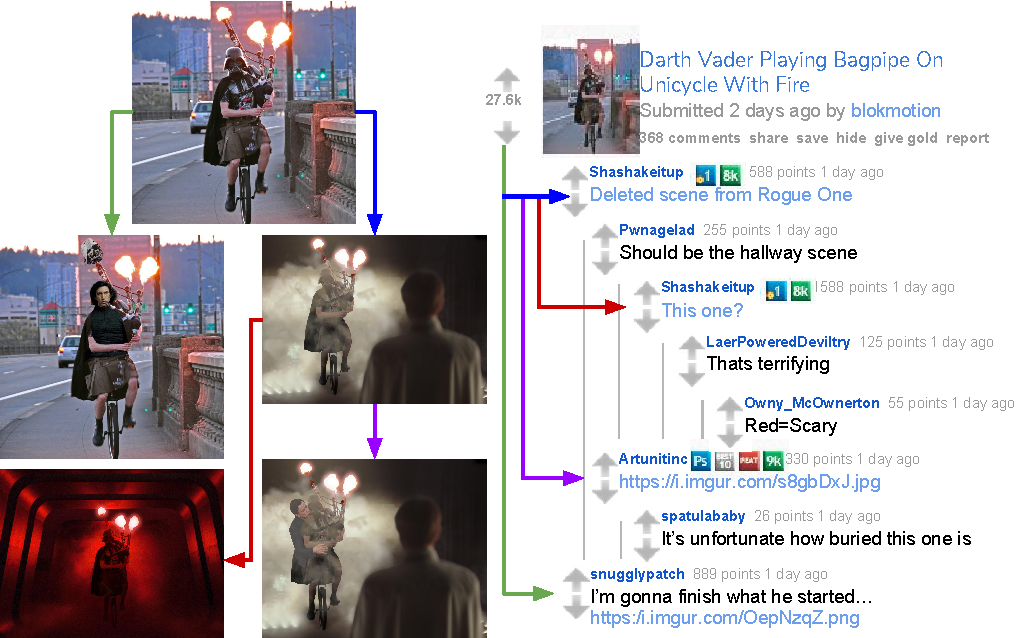
\includegraphics[width=8.5cm]{figures/Reddit_Inference.pdf}
\caption[]{A visualization of how provenance graphs are automatically inferred from a Reddit Photoshop battle instance.
The parent-child behavior of comments (right) can be leveraged to infer the structure of the ground truth provenance graph (left).
The colors of each comment correspond to their respective edge in the graph.} %\footnotemark.}
\label{fig:redditViz}
\end{figure}
%\footnotetext{\url{https://www.reddit.com/r/photoshopbattles/comments/76iqgc/psbattle_darth_vader_playing_bagpipe_on_unicycle/} (accessed on Oct. 31, 2017)}

Because these images are real examples of incremental manipulations, the Reddit dataset accurately represents manipulations and operations performed on images in the wild.
%This is in contrast to all other provenance and phylogeny datasets, which contain only laboratory generated examples.
\RED{To assure the quality of the samples, each graph was manually reviewed. Cases with missing images within the comments or disconnected nodes were automatically discarded.}
In total, the Reddit dataset contains 184 provenance graphs, which together sum up to 10,421 original and composite images.
It will be made available to the public upon the publication of this work.
Similar to the Professional dataset, we are not extending the Reddit dataset with distractors; we perform only oracle-filter analysis over it.


\subsection{Evaluation Metrics}
\label{sec:exp_metrics}

In this work, we adopt the metrics proposed by NIST in~\cite{nist2017dataset} for both the provenance image filtering and graph construction tasks.
In the case of provenance image filtering, we report (for each image query) the CBIR recall of the expected images at three particular cut-off ranks: $R@50$ (the recall considering the top-50 images of the retrieved image rank), $R@100$ (recall for the top-100 images), and $R@200$ (recall for the top-200 images).
Given that recall expresses the percentage of relevant images that are being effectively retrieved, the solution delivering higher recall is considered preferable.

In the case of provenance graph construction, we assess, for each provenance graph that is computed for each query, the $F_1$-measure (\textit{i.e.}, the harmonic mean of precision and recall) of the \emph{retrieved nodes} and of the \emph{retrieved edges} (called \emph{vertex overlap} ($VO$) and \emph{edge overlap} ($EO$), respectively).
Additionally, we report the \emph{vertex and edge overlap} ($VEO$), which is the $F_1$-measure of retrieving both nodes and edges, simultaneously~\cite{Papadimitriou_2010}.
The aim of using such metrics is to assess the overlap between the groundtruth and the constructed provenance graph.
The higher the values of $VO$, $EO$, and $VEO$, the better the quality of the solution.

Finally, in the particular case of $EO$ (and consequently $VEO$), we report the overlap both for directed edges (which are assumed to be the regular situation, and therefore kept for $EO$ and $VEO$), and for undirected edges (when an edge is considered to overlap another one if they connect analogous pairs of nodes, in spite of their orientations).
All aforementioned metrics are assessed through the NIST \emph{MediScore} tool~\cite{nist2017plan}.


\subsection{Large-Scale Infrastructure}
\label{sec:exp_lsi}
% [MAJOR] Moved to here >>>>>>>
%\vspace{0.2cm} 
%\subsubsection{Large-Scale Infrastructure}
%\label{sec:prop_scaling}
\RED{Fig.~\ref{fig:filterPipeline} shows the proposed full pipeline for index \emph{training} and \emph{construction} (previously explained in Sec.~\ref{sec:prop_indxing}).
Index training refers to the process of learning the OPQ rotations and PQ codebooks from a sampling of the local features that are extracted from the target dataset.
We propose to perform such step ahead of time with typical central processing units (CPU).
Index construction, in turn, refers to the computation of the inverted file indices, after properly rotating the previously extracted local features.
The learning of OPQ rotations and PQ codebooks can be done in advance on a CPU, but the construction of indices is well suited to the capabilities of graphical processing units (GPU), allowing for faster computation.}
% TODO: Prof. Rocha's note: Clarify this last sentence. Make it clear what you did in CPU and in GPU.  

\begin{figure}[t]
\centering
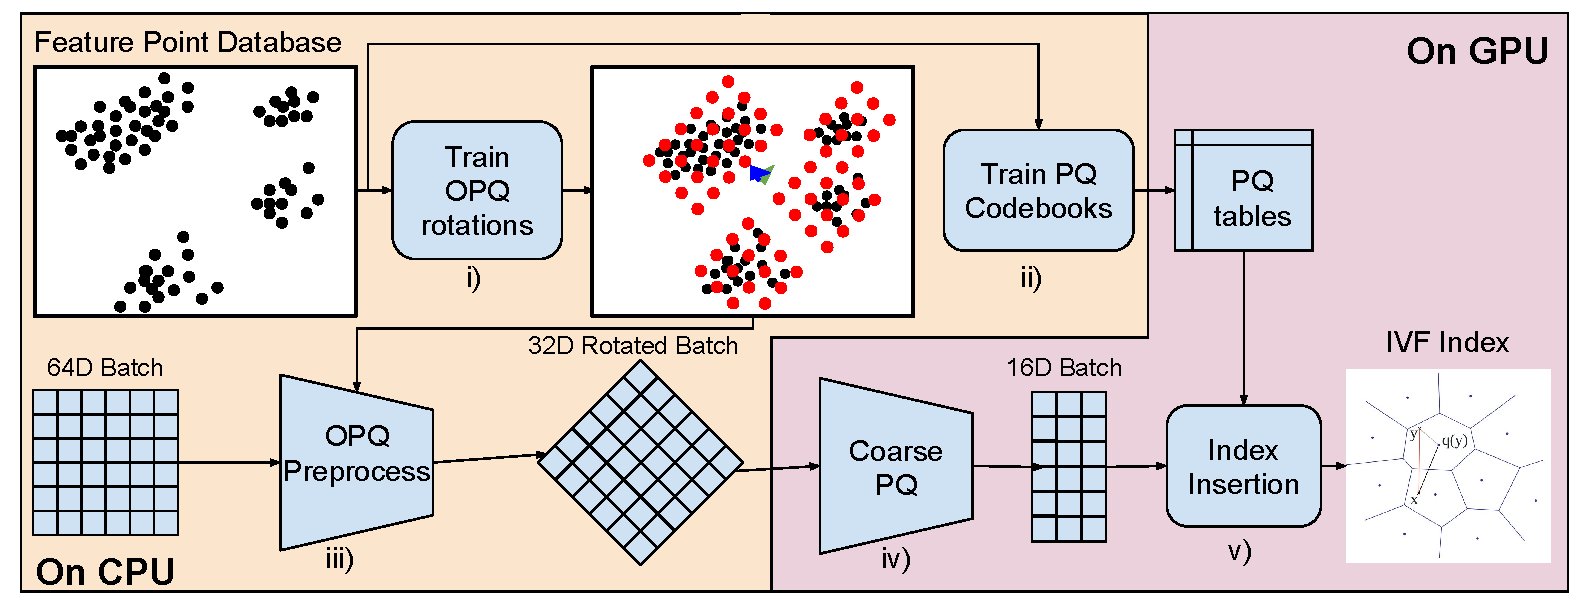
\includegraphics[width=8.7cm]{figures/Indexing_pipeline.pdf}
\caption{Filtering pipeline infrastructure.
The orange area (left) shows computations that are performed on a CPU.
The purple area (right) shows the index ingestion steps that are performed on a GPU.}
\label{fig:filterPipeline}
\end{figure}
% TODO: Prof. Scheirer's note: make on CPU and on GPU labels bold.

\begin{figure}[t]
\centering
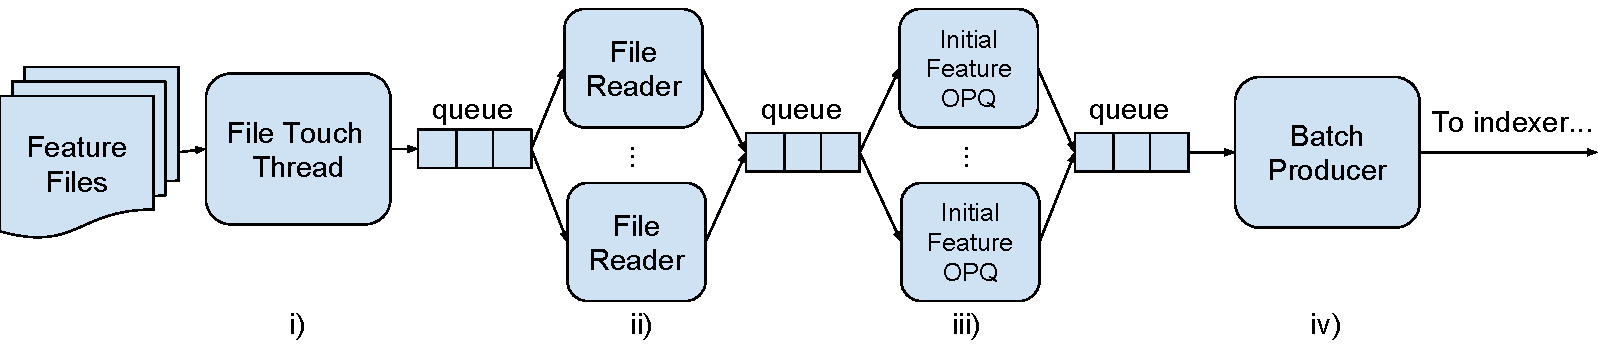
\includegraphics[width=8.7cm]{figures/Fileread_pipeline.pdf}
\caption{
Producer-consumer index ingestion.
Each file contains features for an image.
These file locations are pre-loaded into cache via a rate-limited ``touch" thread, and are read on a producer-consumer multi-threaded basis.}
\label{fig:touchPipeline}
\end{figure}
% TODO: Prof. Scheirer's note: make image texts larger.

\RED{Besides employing GPUs to efficiently build and search an index of over 1 million high-resolution images, additional steps must be taken to increase the pipeline speed.
To date, most indexing algorithms require single large files containing all features to be ingested at once \cite{flann_pami_2014,Attach:binary_matching_crv2012}, either due to implementation choices or algorithm limitations.
The operation of concatenating all features from a set of images into a single file is prohibitively time consuming when dealing with more than a few million interest points.
Because our scenarios require the ingestion of multiple billions of interest points, a different solution must be adopted, in order to avoid the need for file concatenation.
For that, we propose a multi-threaded producer-consumer setup, as shown in Fig.~\ref{fig:touchPipeline}.
In our pipeline, we provide a single feature file per image.
The pipeline begins with the ``touch" thread, which systematically loads image feature file locations into the computer's file system cache, for faster retrieval in later stages.
Then, a reading thread takes touched files and loads them into memory.
A third thread takes sets of loaded feature files and produces feature batches of size $B$ that are optimized in size for GPU ingestion.
The fourth thread applies the initial OPQ pre-processing rotations to the feature set, before sending the final batch to the GPU. Using this method, we are able to process billions of features from high-resolution image datasets orders of magnitudes faster than previous methods.}
% <<<<<<< [MAJOR] Moved to the experimental setup

\subsection{Filtering Setup}
\label{sec:exp_p1}
In all provenance filtering experiments, we either start describing the images with regular 64-dimensional SURF~\cite{Bay:CVIU:2008} interest points, or the distributed approach explained in Sec.~\ref{sec:prop_spread_kp} combined with the SURF detector (namely \emph{DSURF}).
For the regular SURF detector, depending on the experiment, we either extract the top-$2,000$ most responsive interest points (namely \emph{SURF2k}), or the top-$5,000$ most responsive ones (\emph{SURF5k}).
DSURF, in turn, is always described with 5,000 64-dimensional interest points, of which 2,500 regard the top-$2,500$ most responsive ones, and the remaining 2,500 are obtained avoiding overlap, as explained in~Sec.~\ref{sec:prop_spread_kp}.

For the sake of comparison, besides reporting results of the IVFADC system (explained in Sec.~\ref{sec:prop_indxing}), we also report results of the KD-Forest system discussed by Pinto~et~al.~\cite{pinto2017filtering} over the same set of images.
Because the work in~\cite{pinto2017filtering} is not easily scalable beyond 2,000 interest points, with respect to memory footprint, we combine it with SURF2k only (namely \emph{KDF-SURF2k}).

Focusing on the IVFADC approach, we provide combinations of it with all the available low-level descriptor approaches, hence obtaining \emph{IVFADC-SURF2k} (for comparison with KDF-SURF2k), \emph{IVFADC-SURF5k}, and \emph{IVFADC-DSURF}.
Regardless of the descriptors, we are always performing IVFADC with a codebook set size of 32 codes and sub-codebook set size of 96; both values were learned from preliminary experiments as revealing an acceptable trade-off between index building time and size, and final system recall. 
% TODO: Daniel: ask Joel about this codebook and sub-codebook thing. We need to add it to the method explanation (it seems to be missing, for now).
Finally, aiming at evaluating the impact of using iterative filtering (explained in Sec.~\ref{sec:prop_iterative_filtering}), we evaluate variations of the two most robust filtering solutions (namely IVFADC-SURF5k and IVFADC-DSURF) by adding iterative filtering (IF), hence obtaining the \emph{IVFADC-SURF5k-IF} and \emph{IVFADC-DSURF-IF} variations.
% TODO: Daniel: verify with Joel how many iterations we are employing in IF. We should report that here.
% I found it here: Second-tier search utilized a maximum of top 10 result and a minimum of the top 1 images from each first-tier query (chosen using RCMM, Section \ref{lab:filt:SecondTierSearch}.
All filtering methods are tested over the NIST dataset, for each one of its 65 queries.

% TODO: Daniel: describe the computational infrastructure used in the experiments.
% Good Joel's starting points:
% 1. It should be noted that these experiments were performed on a high-performance computing cluster utilizing the Andrew File System (AFS) [60].
% 2. All setups use 5000 descriptors per image and 8 TitanXP GPUs for building the index.
% Add CPU and GPU info (type, number of instances, amount of memory, etc.)


\subsection{Graph Construction Setup}
\label{sec:exp_p2}
As explained in Sec.~\ref{sec:prop:graph_building}, the graph construction task always starts with a given query and its respective rank of potentially related images.
For computing both the GCM-based and MI-based dissimilarity matrices (all explained in Sec.~\ref{sec:prop_dismat}), we either detect and match the top-5,000 most responsive SURF interest points per image, for each image pair, or the top-5,000 largest MSER regions per image, again for each image pair.
As a consequence, we have available four types of dissimilarity matrices, namely GCM-SURF and GCM-MSER (both symmetric), and MI-SURF and MI-MSER (both asymmetric).

The reason for choosing SURF and MSER is related to their potential complementarity: while SURF detects blobs of interest~\cite{Bay:CVIU:2008}, MSER detects the stable complex image regions that are tolerant to various perspective transformations~\cite{Matas_2004}.
Thus, the two methods end up delivering very different sets of interest points.
For extracting feature vectors from both SURF and MSER detected interest points, we compute the 64-dimensional SURF features proposed in~\cite{Bay:CVIU:2008}.
In the particular case of MSER, we compute the SURF features over the minimum enclosing circles that contain each one of the detected MSER image regions.
During the GCM feature matching, we match only interest points of the same type (\textit{i.e.}, we match SURF blobs with only SURF blobs, as well as MSER regions with only MSER regions).

\RED{In the end, we construct the provenance graphs from the four types of dissimilarity matrices using either Kruskal's algorithm over the symmetric GCM-based instances (therefore obtaining undirected graphs), or the herein proposed clustered provenance graph expansion approach, which relies on both GCM- and MI-based instances (obtaining directed graphs). %, as explained in Section~\ref{sec:prop_cluster}.
As a result, we have available, for performing experiments, the following options: \emph{Kruskal-SURF}, obtained from GCM-SURF adjacency matrices, \emph{Kruskal-MSER}, obtained from GCM-MSER adjacency matrices, Cluster-SURF, obtained from both GCM- and MI-SURF matrices, and Cluster-MSER, obtained from both GCM- and MI-MSER matrices.}
% TODO: Daniel: check with Aparna if we are using fusion of methods. If so, we need to explain fusion in the proposed method.

All graph construction methods are tested over the NIST (65 queries), Professional (80 queries), and Reddit (184 queries) datasets.
In the particular case of the NIST dataset, we report both end-to-end and oracle-filter analyses.
Regarding end-to-end analysis, we start with the best top-100 image ranks that were obtained in the former set of provenance image filtering experiments.
As expected, these ranks contain distractors, as well as miss some images related to the query that should be part of the final provenance graph.
With respect to the oracle-filter analysis, the ranks will only contain images related to the query.
%The same aspect will be observed in the case of the Professional and Reddit datasets, which do not count on distractors and, as a result, are submitted to oracle-filter analysis only.
% TODO: Daniel: describe the computational infrastructure used in the experiments.
% Add CPU info (type, number of cores, amount of memory, etc.)
